%%%%%%%%%%%%%%%%%%%%%%%%%%%%%%%%%%%%%%%%%%%%%%%%%%%%%%
% A Beamer template for Ritsumeikan University       %
% Author: Ming-Hao Xu (Xu Minghao)                   %
% Date:   April 2022.                                %
% LPPL Licensed.                                     %
%%%%%%%%%%%%%%%%%%%%%%%%%%%%%%%%%%%%%%%%%%%%%%%%%%%%%%

\documentclass{beamer}
\usepackage{hyperref}
\usepackage[T1]{fontenc}
\usepackage{comment}

% other packages
\usepackage{latexsym,amsmath,xcolor,multicol,booktabs,calligra}
\usepackage{graphicx,pstricks,listings,stackengine,tikz,pgf}

% dummy text; remove it when working on this template
\usepackage{lipsum}
\usepackage{tcolorbox}

\newenvironment{Teorema}[1]{
  \begin{tcolorbox}[colback=blockbackground,colframe=ritsumeikan,title=#1]
}{
  \end{tcolorbox}
}
\newenvironment{Demostracion}[1]{
  \begin{tcolorbox}[colback=blockbackground,colframe=dem,title=#1]
}{
  \end{tcolorbox}
}


\author{Jeisson Jarvey Sánchez Castellanos}
\title{Transformaciones de Möbius:}
\subtitle{Una mirada al análisis complejo}
\institute{
    Universidad Distrital Francisco José de Caldas (UDFJC) \\
    Proyecto Académico de Matemáticas
}
\date{Septiembre, 2022}
\usepackage{Ritsumeikan}

% defs
\def\cmd#1{\texttt{\color{red}\footnotesize $\backslash$#1}}
\def\env#1{\texttt{\color{blue}\footnotesize #1}}
\definecolor{deepblue}{rgb}{0,0,0.5}
\definecolor{deepred}{rgb}{0.6,0,0}
\definecolor{deepgreen}{rgb}{0,0.5,0}
\definecolor{halfgray}{gray}{0.55}

\lstset{
    basicstyle=\ttfamily\small,
    keywordstyle=\bfseries\color{deepblue},
    emphstyle=\ttfamily\color{deepred},    % Custom highlighting style
    stringstyle=\color{deepgreen},
    numbers=left,
    numberstyle=\small\color{halfgray},
    rulesepcolor=\color{red!20!green!20!blue!20},
    frame=shadowbox,
}


\begin{document}

\begin{frame}
    \titlepage
    \begin{figure}[htpb]
        \begin{center}
            \includegraphics[width=0.2\textwidth]{pic/escudo.pdf}
        \end{center}
    \end{figure}
\end{frame}

\begin{frame}
    \tableofcontents[sectionstyle=show,subsectionstyle=show/shaded/hide,subsubsectionstyle=show/shaded/hide]
\end{frame}

\section{Introducción}

\begin{frame}{Introducción}
    \begin{itemize}
        \item $(x,y)=x+iy=z \text{ con } i=\sqrt{-1}$.
        \item $x=\Re(z)$ es la parte real de $z$ y $y=\Im(z)$ es la parte imaginaria.
        \item $\bar{z}=x-iy$.
        \item $|z|=\sqrt{x^2+y^2}$ denotado módulo de $z$ y es la distancia del punto al origen.
        \item 
        \begin{equation*}
            \mathfrak{H} = 
            \begin{pmatrix}
                a & b \\
                c & d \\
            \end{pmatrix}
            \hspace{1cm}
            \mathfrak{C} =
            \begin{pmatrix}
                A & B\\
                C & D\\
            \end{pmatrix}.
        \end{equation*}
    \end{itemize}
\end{frame}

\section{Circunferencias y matrices asociadas}
    
\begin{frame}{Circunferencia y matriz asociada}
    \begin{itemize}
        \item Construcción de ecuación
        \begin{equation*}
            |z-\gamma|^2=\rho^2 \Rightarrow |z-\gamma|^2=(z-\gamma)(\bar{z}-\bar{\gamma})=z\bar{z}-\bar{\gamma}z-\gamma\bar{z}+\gamma\bar{\gamma}.
        \end{equation*}
        \item Ecuación base
        \begin{equation}
            z\bar{z}-\bar{\gamma}z-\gamma\bar{z}+\gamma\bar{\gamma}-\rho^2=0.
            \label{eq:(1)}
        \end{equation}
        \item Ecuación canónica 
        \begin{equation}
            \mathfrak{C}(z,\bar{z})=Az\bar{z}-Bz-C\bar{z}+D=0.
            \label{eq:(2)}
        \end{equation}
        \item Matriz asociada
        \begin{equation}
            \mathfrak{C}=
            \begin{pmatrix}
                A & B \\
                C & D 
            \end{pmatrix}
            \label{eq:(3)}
        \end{equation}
        \item Ecuación \eqref{eq:(1)} es un caso particular de \eqref{eq:(2)}
        \begin{equation}
            B=-A\bar{\gamma};\quad C=-A\gamma = \bar{B}; \quad D = A(\gamma\bar{\gamma}-\rho^2). 
            \label{eq:(4)}
        \end{equation}
    \end{itemize}
\end{frame}
\begin{frame}{Tipos de circunferencias}
    \begin{itemize}
        \item Determinante de la matriz y discriminante de la circunferencia.
        \begin{equation}
            |\mathfrak{C}|=\Delta = AD-BC=AD-|B|^2.
            \label{eq:(5)}
        \end{equation}
        \item En \eqref{eq:(1)} tenemos como discriminante $\delta = -\rho^2$, mientras en \eqref{eq:(2)} tenemos $\Delta = -A^2\rho^2$ por tanto son la misma circunferencia.
        \item $A \neq 0$ y $\Delta < 0$ genera una circunferencia ordinaria.
        \item $A \neq 0$ y $\Delta = 0$ genera un punto circular.
        \item $A \neq 0$ y $\Delta > 0$ genera una circunferencia imaginaria.
        \item Suma de circunferencias.
        \begin{align}
            |\mathfrak{C}|&=
            \begin{vmatrix}
                \lambda_1A_1+\lambda_2A_2 & \lambda_1B_1+\lambda_2B_2\\
                \lambda_1C_1+\lambda_2C_2 &
                \lambda_1D_1+\lambda_2D_2
            \end{vmatrix}\\
            &=\Delta_1\lambda^2_1+2\Delta_{12}\lambda_1\lambda_2+\Delta_2\lambda^2_2.
            \label{eq:(9)}
        \end{align}
    \end{itemize}
\end{frame}
\begin{frame}{Inversión}
    \begin{itemize}
        \item Circunferencia de $z$ y $z^*$
        \begin{equation}
            Az^*\bar{z}+Bz^*+C\bar{z}+D=\mathfrak{C}(z^*,\bar{z}).
            \label{eq:(15)}
        \end{equation}
        \item Definición de $z^*$.
        \begin{align}
            z^*&=-\frac{C\bar{z}+D}{A\bar{z}+B}\notag\\
            &=\gamma+\frac{\rho^2}{\bar{z}-\bar{\gamma}}.
            \label{eq:(16)}
        \end{align}
        \item Queremos que  $z^*=f(z)$ sea una correspondencia uno a uno.
        \begin{equation}
            f(\gamma)=\infty
            \label{eq:(17)}
        \end{equation}
        \begin{equation}
            f(\infty)=\gamma,
            \label{eq:(18)}
        \end{equation}
    \end{itemize}
\end{frame}

\begin{frame}{Teoremas}
    \begin{Teorema}{Teorema}
        Cada inversión lleva circunferencias en circunferencias, circunferencias reales (incluidas las rectas) en circunferencias reales y circunferencias imaginarias en circunferencias imaginarias.
    \end{Teorema}
    \begin{Demostracion}{Demostración}
        Evaluamos dos casos
        \begin{itemize}
            \item Recta.
            \begin{equation*}
                Bz^*+c\bar{z^*}+D=0 \Rightarrow \Delta=-BC=|B|^2 \Rightarrow \Delta^*=\Delta
            \end{equation*}
        \end{itemize}
    \end{Demostracion}
\end{frame}

\begin{frame}{Demostración}
    \begin{Demostracion}{Demostración}
        \begin{itemize}
            \item Circunferencia (real o imaginaria)\\
            De \eqref{eq:(16)} tenemos que $z^*=1/\bar{z}$, al reemplazar en \eqref{eq:(2)} $z$ por $1/\bar{z^*}$ y al multiplicar por $z^*\bar{z^*}$ obtenemos
            \begin{equation}
                z^*\bar{z^*}\mathfrak{C}\left(\frac{1}{\bar{z^*}},\frac{1}{z^*}\right)=Dz^*\bar{z^*}+Bz^*+C\bar{z^*}+A=0,
                \label{eq:(19)}
            \end{equation}
            y su discriminante cumple que $\Delta^*=\Delta$.
        \end{itemize}
    \end{Demostracion}
\end{frame}

\begin{frame}{Relación cruzada}
    \begin{itemize}
        \item Relación simple.
        \begin{equation}
            (z_1;z_2,z_3) = \left\{
            \begin{array}{lcc}
               \frac{z_1-z_2}{z_1-z_3}  & \text{ sí } & z_3 \neq z_1  \\
                 \infty & \text{ sí } & z_1=z_3
            \end{array}
            \right.
            \label{eq:(34)}
        \end{equation}
        \item Relación cruzada.
        \begin{equation}
            (z_1,z_2;z_3,z_4) = \frac{(z_1-z_3)(z_2-z_4)}{(z_1-z_4)(z_2-z_3)}
            \label{eq:(35)}
        \end{equation}
    \end{itemize}
\end{frame}

\section{Transformaciones de Möbius}
\subsection{Propiedades básicas}

\begin{frame}{Definición y caso constante}
    \begin{itemize}
        \item Definición.
        \begin{equation}
            Z=\mathfrak{H}(z)=\frac{az+b}{cz+d}.
            \label{eq:(22)}
        \end{equation}
        \item Matriz asociada.
        \begin{equation*}
            \mathfrak{H}=
            \begin{pmatrix}
                a & b\\
                c & d
            \end{pmatrix}.
        \end{equation*}
        \item Su determinante es
        \begin{equation*}
            |\mathfrak{H}|=\delta=ad-bc
        \end{equation*}
        \item $\delta \neq 0$ ya que de no serlo
        \begin{align*}
            Z&=\frac{\frac{bc}{d}z+b}{cz+d}\\
            &=\frac{b}{d}.
        \end{align*}
        lo que significa que es constante.
    \end{itemize}
\end{frame}
\begin{frame}{Linealidad y bilinealidad}
    \begin{itemize}
        \item Definimos
        \begin{equation*}
            z=\frac{z_1}{z_2} \quad Z=\frac{Z_1}{Z_2}.
        \end{equation*}
        \item De la relación \eqref{eq:(22)} podemos obtener
        \begin{align}
            \frac{1}{q}Z_1&=az_1+bz_2\notag\\
            \frac{1}{q}Z_2&=cz_1+dz_2
            \label{eq:(23)}
        \end{align}
        \item De aquí se deduce
        \begin{equation*}
             \frac{Z_1}{Z_2}=\frac{az_1+bz_2}{cz_1+dz_2}.
        \end{equation*}
        esto es una transformación lineal homogénea en variables $z_1$ y $z_2$
        \item finalmente es llamada transformación bilineal
        \begin{equation}
            czZ+dZ-az-b=0.
            \label{eq:(25)}
        \end{equation}
    \end{itemize}
\end{frame}

\begin{frame}{Linealidad y bilinealidad}
    \begin{itemize}
        \item luego hacemos uso de la matriz $\mathfrak{H}$ y la siguiente notación columna
        \begin{equation*}
            \mathfrak{z}=\frac{z_1}{z_2}, \quad \mathfrak{Z}=\frac{Z_1}{Z_2}.
        \end{equation*}
        \item De manera que \eqref{eq:(23)} se puede ver de la siguiente manera
        \begin{equation}
            \mathfrak{Z}=q\mathfrak{H}\mathfrak{z}.
            \label{eq:(24)}
        \end{equation}
    \end{itemize}
\end{frame}

\subsection{Grupo de las Transformaciones de Möbius}

\begin{frame}{Grupo de las transformaciones de Móbius}
    \begin{itemize}
        \item Sean $\mathfrak{H}_1,\mathfrak{H}_2$ dos transformaciones de Möbius
        \begin{equation*}
            \mathfrak{H}_1=
            \begin{pmatrix}
                a_1 & b_1\\
                c_1 & d_1
            \end{pmatrix}
            \text { y } 
            \quad
            \mathfrak{H}_2=
            \begin{pmatrix}
                a_2 & b_2\\
                c_2 & d_2
            \end{pmatrix}.
        \end{equation*}
        \item Llevadas en sucesión
        \begin{equation}
            Z=\mathfrak{H}_2(\mathfrak{H}_1(z)).
            \label{eq:(26)}
        \end{equation}
        \item es a su vez una transformación de Möbius
        \begin{equation*}
            Z=\frac{a_2\mathfrak{H}_1(z)+b_2}{c_2\mathfrak{H}_1(z)+d_2}=\frac{(a_1a_2+b_2c_1)z+a_2b_1+b_2d_1}{(c_2a_1+d_2c_1)z+c_2b_1+d_2d_1}.
        \end{equation*}
        \item Notese que la matriz puede verse como el producto de las otras matrices
        \begin{equation}
            \mathfrak{H}_3=\mathfrak{H}_2\mathfrak{H}_1=
            \begin{pmatrix}
                a_2a_1+b_2c_1 & a_2b_1+b_2d_1\\
                c_2a_1+d_2c_1 & c_2b_1+d_2d_1
            \end{pmatrix}.
            \label{eq:(27)}
        \end{equation}
    \end{itemize}
\end{frame}

\begin{frame}{Grupo de las transformaciones de Móbius}
    \begin{itemize}
        \item La función producto \eqref{eq:(26)} es con certeza no constante y su inversa a su vez es una transformación de Möbius
        \begin{equation}
            z=(H)^{-1}(Z)=\frac{dZ-b}{-cZ+a}
            \label{eq:(28)}
        \end{equation}
    \end{itemize}
    \begin{Teorema}{Teorema}
        El sistema de todas las transformaciones de Möbius es un grupo con la composición funcional como un grupo multiplicativo.
    \end{Teorema}
\end{frame}

\subsection{Transformaciones de Möbius de tipo simple}

\begin{frame}{Transformaciones de tipo simple}
    \begin{itemize}
        \item Sí $c=0$ podemos asumir que $d=1$, con lo cual $\mathfrak{H}(z)$ se puede ver como una función lineal
        \begin{equation*}
            Z=az+b.
        \end{equation*}
        \item Sí $c\neq0$ la fórmula \eqref{eq:(22)} puede ser escrita de la siguiente forma haciendo la división de polinomios
        \begin{equation}
            Z = \frac{a}{c}-\frac{\delta}{c}\frac{1}{cz+d}. 
            \label{eq:(29)}
        \end{equation}
        De este modo una transformación de Möbius aparece como un producto de transformaciones de Möbius de tipo simple
    \end{itemize}
\end{frame}
\begin{frame}{Translación y Rotación}
    \begin{Teorema}{Translación}
        \begin{equation}
            Z=z+b \quad \text{ con matriz asociada } \mathfrak{I}_b=\begin{pmatrix}
                1 & b\\
                0 & 1
            \end{pmatrix}
            \text{con } b\in \mathbb{C}-\{0\}
            \label{eq:(30)}
        \end{equation}
    \end{Teorema}
    \begin{Teorema}{Rotación}
        \begin{equation}
            Z=e^{i\alpha}z \quad \text{ con matriz asociada }\mathfrak{R}_\alpha =
            \begin{pmatrix}
                e^{i\alpha} & 0\\
                0 & 1
            \end{pmatrix}
            \label{eq:(31)}
        \end{equation}
    \end{Teorema}
\end{frame}

\begin{frame}{Translación}
    \begin{figure}[!ht]
        \begin{center}
            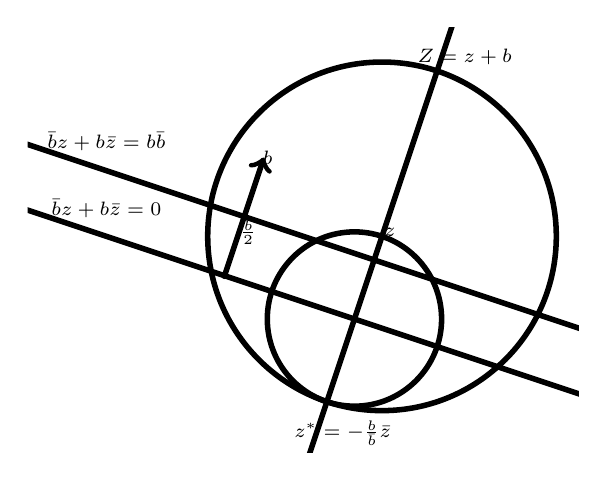
\begin{tikzpicture}[scale=0.5]
                \clip(-5,-4.5) rectangle (9,6.3);
                    \draw [->,line width=2pt] (0,0) -- (1,3);
                    \draw [line width=2pt,domain=-6.121042670321929:11.004975779907687] plot(\x,{(-0--1*\x)/-3});
                    \draw [line width=2pt,domain=-6.121042670321929:11.004975779907687] plot(\x,{(--11-3*\x)/-1});
                    \draw [line width=2pt] (3.3,-1.1) circle (2.213594362117866cm);
                    \draw [line width=2pt,domain=-6.121042670321929:11.004975779907687] plot(\x,{(-5--1*\x)/-3});
                    \draw [line width=2pt] (4,1) circle (4.427188724235733cm);
                    \begin{scriptsize}
                    \draw [fill=black] (0,0) circle (2pt);
                    \draw [color=black] (1.1,3) node {$b$};
                    \draw[color=black] (0.6,1.1) node {$\frac{b}{2}$};
                    \draw [fill=black] (0.5,1.5) circle (2pt);
                    \draw [fill=black] (4,1) circle (2.5pt);
                    \draw[color=black] (4.2,1.1) node {$z$};
                    \draw[color=black] (-3,1.7) node {$\bar{b}z+b\bar{z}=0$};
                    \draw[color=black] (-3,3.4) node {$\bar{b}z+b\bar{z}=b\bar{b}$};
                    \draw [fill=black] (2.6,-3.2) circle (2pt);
                    \draw [fill=black] (2.6,-3.2) circle (2pt);
                    \draw[color=black] (3,-4) node {$z^*=-\frac{b}{\bar{b}}\bar{z}$};
                    \draw [fill=black] (5.4,5.2) circle (2pt);
                    \draw[color=black] (6.1,5.547002568071058) node {$Z=z+b$};
                    \end{scriptsize}
                \end{tikzpicture}
        \end{center}
        \caption{Translación del punto $z$ al punto $Z=z+b$}
        \label{fig:translacion}
        \end{figure}
\end{frame}

\begin{frame}{Rotación}
    \begin{figure}[ht]
        \begin{center}
            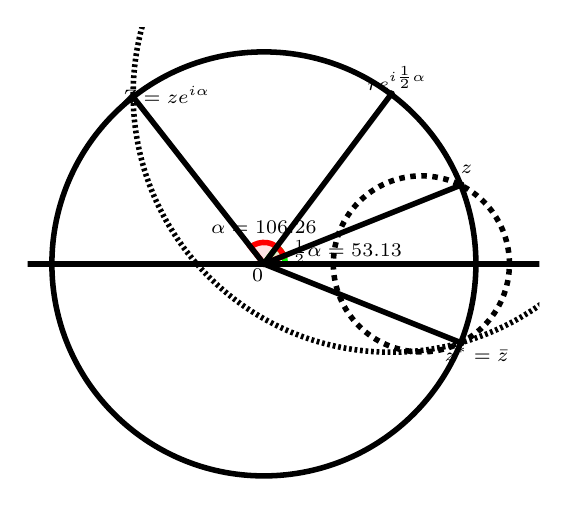
\begin{tikzpicture}[scale=0.5]
                \clip(-6,-6) rectangle (7,6);
                \draw [shift={(0,0)},line width=2pt,color=green,fill=green,fill opacity=0.10000000149011612] (0,0) -- (0:0.5454545454545452) arc (0:53.13010235415597:0.5454545454545452) -- cycle;
                \draw [shift={(0,0)},line width=2pt,color=red,fill=red,fill opacity=0.1] (0,0) -- (21.80140948635181:0.5454545454545452) arc (21.80140948635181:128.06161419466378:0.5454545454545452) -- cycle;
                \draw [line width=2pt] (0,0) circle (5.385164807134505cm);
                \draw [line width=2pt,dotted] (4,0) circle (2.23606797749979cm);
                \draw [line width=2pt] (0,0)-- (5,2);
                \draw [line width=2pt] (0,0)-- (5,-2);
                \draw [line width=2pt] (0,0)-- (3.231098884280703,4.308131845707603);
                \draw [line width=2pt,dash pattern=on 1pt off 1pt] (3.231098884280703,4.308131845707603) circle (6.5514531624688725cm);
                \draw [line width=2pt] (-3.32,4.24)-- (0,0);
                \draw [line width=2pt,domain=-8.798181818181813:8.98363636363636] plot(\x,{(-0-0*\x)/-4});
                \begin{scriptsize}
                \draw [fill=black] (0,0) circle (2pt);
                \draw[color=black] (-0.1618181818181803,-0.3) node {$0$};
                \draw [fill=black] (5,2) circle (2.5pt);
                \draw[color=black] (5.1472727272727266,2.3945454545454523) node {$z$};
                \draw [fill=black] (5,-2) circle (2.5pt);
                \draw[color=black] (5.4,-2.2963636363636346) node {$z^*=\bar{z}$};
                \draw [fill=black] (3.231098884280703,4.308131845707603) circle (2.5pt);
                \draw[color=black] (3.3836363636363638,4.70363636363636) node {$re^{i\frac{1}{2}\alpha}$};
                \draw[color=black] (2.1,0.3) node {$\frac{1}{2}\alpha = 53.13$};
                \draw [fill=black] (-3.32,4.24) circle (2pt);
                \draw[color=black] (-2.5,4.3) node {$Z=ze^{i\alpha}$};
                \draw[color=black] (0,0.94) node {$\alpha = 106.26$};
                \end{scriptsize}
            \end{tikzpicture}
        \end{center}
        \caption{Rotación del punto $z$ al punto $Z=ze^{i\alpha}$}
        \label{fig:rotacion}
        \end{figure}
\end{frame}

\begin{frame}{Dilatación y Reciprocidad}
    \begin{Teorema}{Dilatación}
        \begin{equation}
            Z=\rho z \quad \text{ con matriz asociada }\mathfrak{D}_\rho =
            \begin{pmatrix}
                \rho & 0\\
                0 & 1
            \end{pmatrix}
            \label{eq:(32)}
        \end{equation}
    \end{Teorema}
    \begin{Teorema}{Reciprocidad}
        \begin{equation}
            Z=\frac{1}{z} \text{con matriz asociada } \mathfrak{R}=
            \begin{pmatrix}
                0 & 1\\
                1 & 0
            \end{pmatrix}
            \label{eq:(33)}
        \end{equation}
    \end{Teorema}
\end{frame}
\subsection{Combinación de tipo simple}
\begin{frame}{Propiedades}
    \begin{itemize}
        \item Combinación de Transformación lineal
        \begin{equation*}
            \mathfrak{H}=\mathfrak{I}_b\mathfrak{R}_\alpha\mathfrak{D}_{|a|},
        \end{equation*}
        \item Caso no lineal
        \begin{equation*}
            \mathfrak{H}=\mathfrak{I}_{a/c}\mathfrak{D}_{|\delta/c|}\mathfrak{R}\mathfrak{I}_{d}\mathfrak{D}_{|c|}\mathfrak{R}_{\gamma}
        \end{equation*}
    \end{itemize}
\end{frame}

\begin{frame}{Teoremas}
    \begin{Teorema}{Teorema}
        Cada transformación de Möbius es una aplicación del plano $z$ completo en el plano $Z$ completo. Transforma circunferencias en circunferencias, circunferencias reales en circunferencias reales (incluyendo rectas) e imaginarias en imaginarias
    \end{Teorema}
    \begin{Teorema}{Teorema}
        Toda transformación de Möbius $\mathfrak{H}$ conserva la orientación de cualquier circunferencia que no contenga el polo de $\mathfrak{H}$. Sí $\mathfrak{C}$ contiene el polo de $\mathfrak{H}$ entonces la imagen $\mathfrak{C}_1$ de $\mathfrak{C}$ tiene su orientación opuesta a la de $\mathfrak{C}$. Sí el polo de $\mathfrak{H}$ se encuentra en $\mathfrak{C}$, entonces la imagen de $\mathfrak{C}$ es una línea recta.
    \end{Teorema}
\end{frame}

\begin{frame}{Teoremas}
    \begin{Teorema}{Teorema}
        Sean $z_1,z_2,z_3,z_4$ cuatro puntos cualesquiera del plano completo de los cuales tres no colineales. Sean $\mathfrak{H}$ una transformación de Möbius y $Z_j=\mathfrak{H}(z_j)$ con $j=1,2,3,4$ entonces
    \begin{equation*}
        (Z_1,Z_2;Z_3,Z_4)=(z_1,z_2;z_3,z_4)
    \end{equation*}
    Más brevemente, la relación cruzada es un invariante (invariante de cuatro puntos) del grupo de todas las transformaciones de Möbius
    \end{Teorema}
\end{frame}

\begin{frame}{Ejemplo}
    \begin{itemize}
        \item Supongamos que tenemos cuatro puntos en el plano complejo:
            \begin{equation*}
                z_1,\quad
                z_2, \quad
                z_3, \quad
                z_4.
            \end{equation*}
            \item Aplicamos inversión a cada uno de los puntos $z_1, z_2, z_3, z_4$ para obtener
            \begin{equation*}
                Z_1=z_1^*, \quad Z_2=z_2^*, \quad Z_3=z_3^*, \quad Z_4=z_4^*,    
            \end{equation*}
            \item por definición tenemos que 
            \begin{align*}
                z^*_j=\gamma_0\frac{\rho_0^2}{\bar{z_j}-\bar{\gamma_0}},
            \end{align*}
            \item esto quiere decir
            \begin{align*}
                z^*_j-z^*_k=\rho_0^2\frac{\bar{z_k}-\bar{z_j}}{(\bar{z_j}-\bar{\gamma_0})(\bar{z_k}-\bar{\gamma_0})}.
            \end{align*}
    \end{itemize}
\end{frame}

\begin{frame}{Ejemplo}
    \begin{itemize}
        \item y por tanto al hacer los respectivo procedimientos
            \begin{align*}
                (z_1^*,z_2^*;z_3^*,z_4^*)
                &=\frac{\left(\rho_0^2\frac{\bar{z_3}-\bar{z_1}}{(\bar{z_1}-\bar{\gamma_0})(\bar{z_3}-\bar{\gamma_0})}\right)\left(\rho_0^2\frac{\bar{z_4}-\bar{z_2}}{(\bar{z_2}-\bar{\gamma_0})(\bar{z_4}-\bar{\gamma_0})}\right)}{\left(\rho_0^2\frac{\bar{z_4}-\bar{z_1}}{(\bar{z_1}-\bar{\gamma_0})(\bar{z_4}-\bar{\gamma_0})}\right)\left(\rho_0^2\frac{\bar{z_3}-\bar{z_2}}{(\bar{z_2}-\bar{\gamma_0})(\bar{z_3}-\bar{\gamma_0})}\right)}\\
                &=\overline{(z_1,z_2;z_3,z_4)}.
            \end{align*}
            Al hacer nuevamente la inversión repetimos el mismo proceso obteniendo un doble conjugado, con lo cual se puede ver que es invariante.
    \end{itemize}
\end{frame}

\section{Conclusiones}

\begin{frame}
    La demostración de los tres teoremas anteriores nos dejan 3 conclusiones claras
    \begin{enumerate}
        \item Las transformaciones de Möbius conforman un grupo multiplicativo con la composición como operación binaria.
        \item Las transformaciones de Möbius transforman circunferencias a circunferencias, bien sean líneas, circunferencias reales o imaginarias.
        \item Toda transformación de Möbius conserva la orientación de cualquier circunferencia que no contenga el polo de la circunferencia transformada.
        \item La relación cruzada es un invariante en el grupo de las transformaciones de Möbius.
    \end{enumerate}
\end{frame}

\section{References}
\begin{frame}[allowframebreaks]
    \bibliography{ref}
    \bibliographystyle{ieeetr}
    \nocite{*} % used here because no citation happens in slides
    % if there are too many try use:
    % \tiny\bibliographystyle{alpha}
\end{frame}

\begin{frame}
    \begin{center}
        {\Huge\calligra Gracias}
        \begin{center}
            \includegraphics[width=0.2\textwidth]{pic/logo.png}
        \end{center}
    \end{center}
\end{frame}
\end{document}